\chapter{Análisis y Especificación de Requisitos}
\label{cap:analisisRequisitos}

Este capítulo detalla los requisitos y el público objetivo de la aplicación bajo un enfoque de Diseño Centrado en el Usuario (DCU). Mediante el uso de \textit{Personas} e \textit{Historias de Usuario}, se pasa de una problemática inicial a funcionalidades claras, facilitando el análisis del problema hasta la definición de los hitos de desarrollo que han existido durante la evolución del proyecto.

\section{Definición del Problema}

El diseño de la aplicación \textit{ClimbIt} busca solventar un conjunto de carencias detectadas en el panorama actual de la escalada en rocódromo, como se expuso en el Capítulo \ref{cap:estadoDelArte}. Para que el análisis de requisitos sea efectivo, es necesario desgranar el problema en tres grandes bloques que la aplicación debe mitigar:

\begin{enumerate}
    \item \textbf{Dificultad en el seguimiento del progreso:} La falta de un estándar en las escalas de dificultad y el cambio de rutas constante de los rocódromos hacen que el registro manual sean métodos ineficaces, causando al escalador frustración y desembocando en un abandono del seguimiento.
    \item \textbf{Carencia de motivación a largo plazo:} El progreso físico y técnico en la escalada es muy lento y con largas fases de estancamiento por lo que sin una plataforma que aplique mecánicas de gamificación para visualizar logros a corto o medio plazo y fomente la competitividad, la retención del escalador baja.
    \item \textbf{Desconexión en la gestión deportiva:} Los \textit{route-setters} invierten un gran esfuerzo en renovar los muros, pero carecen de una vía sencilla para registrarlos y para obtener \textit{feedback} (estadísticas de popularidad, valoraciones de dificultad) por parte de la comunidad del rocódromo.
\end{enumerate}

\section{Personas}

Para asegurar que las funcionalidades a desarrollar cubren los problemas expuestos, se hace uso de la técnica de \textit{Personas} \citep{losana2021systematic}. A continuación, se presentan dos perfiles ficticios, pero representativos, basados en el público objetivo, que encarnan los dos roles principales de la aplicación: el escalador y el gestor del rocódromo.

\subsection{Persona 1: Klaudia, Escaladora Constante}

Se presenta el perfil de Klaudia en la figura~\ref{fig:Klaudia}, una escaladora que frecuenta el rocódromo y desea registrar su progreso y mantenerse motivada.

\begin{figure}[h!]
    \centering
    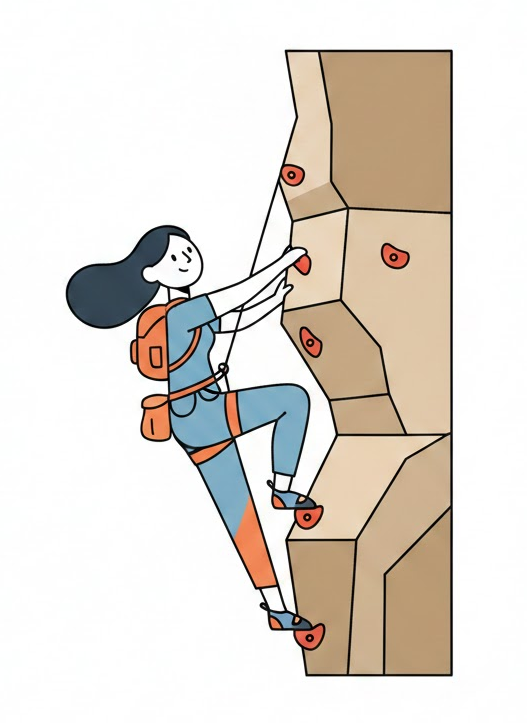
\includegraphics[width=0.4\textwidth]{./Imagenes/Fuentes/klaudia.png} 
    \caption{Perfil de la persona Klaudia}
    \label{fig:Klaudia}
\end{figure}

\begin{itemize}
    \item \textbf{Perfil:} Klaudia, escaladora habitual, 24 años.
    \item \textbf{Nivel de escalada:} Intermedio (6a - 6c).
    \item \textbf{Frecuencia:} Va a entrenar al rocódromo 2-3 veces por semana.
    \item \textbf{Biografía:} Klaudia se inició en la escalada hace un par de años y se ha convertido en su principal pasatiempo y aunque no es profesional, se toma en serio su progreso. Conoce bien las instalaciones y se da cuenta rápidamente cuando las rutas cambian. Le encanta la sensación de superar rutas por encima de su nivel, pero le frustra no ver de forma clara su progreso a lo largo del tiempo.
    \item \textbf{Metas y Motivaciones:}
    \begin{itemize}
        \item Quiere tener un registro de las rutas que ha completado para visualizar su progreso.
        \item Disfruta socializando en el rocódromo y le gusta compartir sus logros con sus amigos.
        \item Busca una competir con algún compañero que la anime a esforzarse más en cada sesión.

    \end{itemize}

    \item \textbf{Frustraciones y Puntos de Dolor:}
    \begin{itemize}
        \item Resulta tedioso llevar un registro manual y a menudo olvida qué rutas ha completado.
        \item Se siente estancada porque no tiene información para analizar sus puntos fuertes y débiles.
        \item No existe una forma fácil de comparar su rendimiento con el de sus compañeros de rocódromo.
    \end{itemize}

    \item \textbf{Relación con la aplicación (\textit{ClimbIt}):} Klaudia es la usuaria final ideal de forma que empleará la aplicación en cada sesión para actualizar sus ascensos, consultar sus estadísticas personales y participar en los rankings mensuales (\textit{leaderboards}).
\end{itemize}

\subsection{Persona 2: Víctor, Gestor del Rocódromo}

Se presenta el perfil de Víctor en la figura~\ref{fig:Victor}, un \textit{route-setter} cuyo objetivo es gestionar eficientemente el muro y dinamizar a su comunidad.

\begin{figure}[h!]
    \centering
    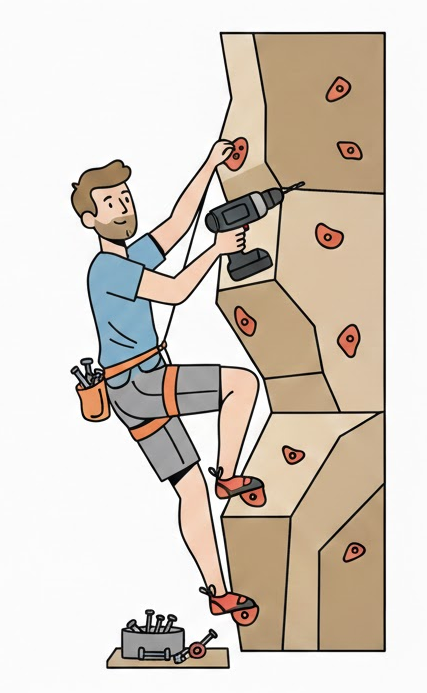
\includegraphics[width=0.4\textwidth]{./Imagenes/Fuentes/victor.png} 
    \caption{Perfil de la persona Víctor}
    \label{fig:Victor}
\end{figure}

\begin{itemize}
    \item \textbf{Perfil:} Víctor, \textit{route-setter} principal y propietario, 42 años.
    \item \textbf{Rol:} Responsable del diseño y renovación de las rutas.
    \item \textbf{Biografía:} Víctor lleva más de una década gestionando su centro siendo su prioridad mantener el rocódromo vivo y desafiante, cambiando sectores del muro semanalmente. Busca que su rocódromo ofrezca un valor añadido comparado con la competencia.
    \item \textbf{Metas y Motivaciones:}
    \begin{itemize}
        \item Ofrecer la mejor experiencia y servicios a los clientes de su rocódromo.
        \item Recibir \textit{feedback} sobre la calidad y la dificultad real de las rutas que equipa.
        \item Crear a una comunidad unida en torno a su rocódromo.
    \end{itemize}
    \item \textbf{Frustraciones y Puntos de Dolor:}
    \begin{itemize}
        \item Ignora de forma objetiva qué rutas son las más populares o cuáles no gustan.
        \item Echa en falta una plataforma para registrar todas las nuevas rutas.
    \end{itemize}
    \item \textbf{Relación con la aplicación (\textit{ClimbIt}):} Víctor utilizará el panel de gestión para mantener actualizadas las rutas del rocódromo y ClimbIt actuará como una herramienta de gestión que le proporcionará un valor añadido a su rocódromo.
\end{itemize}

\section{Especificación de Funcionalidades (Historias de Usuario)}

Una vez comprendido los usuarios, los requisitos del sistema se han especificado mediante Historias de Usuario. En esta sección se listan los identificadores y títulos de las funcionalidades completadas en el desarrollo de ClimbIt extraídas del \textit{Product Backlog} y agrupadas por temática. 

Dado que la descripción y los criterios de aceptación de todas las Historias de Usuario son extensas se podrán ver en detalle en el siguiente enlace a GitHub projects \footnote{Enlace al listado de HUs: https://github.com/users/Melendo/projects/7/views/10} para facilitar la lectura y fluidez de este documento.

\subsection{Autenticación y Gestión de Perfil}
Historias orientadas al acceso al sistema y la personalización de la cuenta:
\begin{itemize}
    \item \textbf{CI-1:} Iniciar sesión con correo y contraseña.
    \item \textbf{CI-2:} Cerrar sesión.
    \item \textbf{CI-10:} Registro con correo electrónico.
    \item \textbf{CI-47:} Tutorial al registrarse (\textit{Onboarding}).
    \item \textbf{CI-3:} Mostrar información básica del perfil.
    \item \textbf{CI-21:} Modificar descripción del perfil.
    \item \textbf{CI-22:} Cambiar foto de perfil entre opciones predefinidas.
    \item \textbf{CI-23:} Mostrar estadísticas básicas del perfil.
    \item \textbf{CI-24:} Cambiar apodo.
    \item \textbf{CI-25:} Mostrar descripción del perfil.
    \item \textbf{CI-45:} Estadísticas de escalador filtradas por rocódromo específico.
\end{itemize}

\subsection{Social y Comunidad}
Historias centradas en la interacción entre los usuarios (sistema \textit{Relatedness}):
\begin{itemize}
    \item \textbf{CI-13:} Buscar usuario por apodo.
    \item \textbf{CI-14:} Enviar solicitud de amistad.
    \item \textbf{CI-15:} Gestión de solicitudes recibidas.
    \item \textbf{CI-16:} Mostrar listado de amigos.
    \item \textbf{CI-17:} Eliminar amigo.
    \item \textbf{CI-44:} Ver perfil público de un amigo.
    \item \textbf{CI-46:} \textit{Leaderboard} mensual de rutas escaladas entre amigos.
    \item \textbf{CI-28:} Crear grupo de escaladores.
    \item \textbf{CI-29:} Enviar invitación a grupo.
    \item \textbf{CI-30:} Gestionar invitación de unión a grupo.
    \item \textbf{CI-32:} Visualizar estadísticas de los miembros del grupo.
\end{itemize}

\subsection{Rocódromos}
Historias orientadas a la exploración de centros y a la administración general:
\begin{itemize}
    \item \textbf{CI-8:} Escalador se suscribe a rocódromo.
    \item \textbf{CI-9:} Escalador se da de baja de un rocódromo.
    \item \textbf{CI-11:} Mostrar listado de ``Mis rocódromos''.
    \item \textbf{CI-12:} Buscador básico de rocódromos.
    \item \textbf{CI-18:} Modificar información básica de rocódromo.
    \item \textbf{CI-26:} Añadir sistemas/tipos de dificultad personalizados del rocódromo.
    \item \textbf{CI-37:} Mostrar información básica del centro.
\end{itemize}

\subsection{Zonas}
Historias relacionadas con la estructuración del espacio del rocódromo:
\begin{itemize}
    \item \textbf{CI-4:} Mostrar mapa básico de zonas de rocódromo.
    \item \textbf{CI-38:} Mostrar zonas con indicador de porcentaje de completado.
    \item \textbf{CI-39:} Mostrar mapa dinámico e interactivo de la zona.
\end{itemize}

\subsection{Rutas}
Historias relativas a la interacción directa con las vías y bloques:
\begin{itemize}
    \item \textbf{CI-5:} Mostrar mapa de rutas dentro de una zona.
    \item \textbf{CI-6:} Listado básico de rutas.
    \item \textbf{CI-7:} Cambiar estado de ascenso de una ruta (\textit{flash}, completado, proyecto).
    \item \textbf{CI-19:} Añadir nueva ruta al rocódromo.
    \item \textbf{CI-20:} Modificar los parámetros de una ruta existente.
    \item \textbf{CI-27:} Eliminar (borrado lógico) una ruta del rocódromo.
    \item \textbf{CI-40:} Filtros de búsqueda por dificultad en zona.
    \item \textbf{CI-41:} Mostrar información avanzada e imágenes de la ruta.
    \item \textbf{CI-42:} Valorar ruta mediante un sistema de estrellas.
    \item \textbf{CI-43:} Visualizar métricas de ascenso segmentadas por dificultad.
\end{itemize}

\section{Roles del Sistema}

Orientándose a una visión técnica del proyecto se ha definido un modelo de permisos basado en cuatro roles principales, cada uno de estos con un nivel de autorización y acceso a las funcionalidades dentro de la plataforma:

\subsection{Escalador}
Es el rol base que representa al usuario final, siendo su objetivo principal es registrar sus actividades y participar en la comunidad. Tiene permisos de lectura sobre la información pública de los rocódromos y permisos de escritura sobre sus datos personales y entre sus funciones se encuentran la gestión de su perfil, la interacción social, el registro de ascensos y la consulta de clasificaciones y estadísticas.

\subsection{Gestor de Rocódromo}
Rol organizativo asignado a los trabajadores o \textit{route-setters} de un centro específico de manera que heredan los permisos básicos de un escalador, sumando privilegios de gestión de las rutas en sus rocódromos asignados (crear, modificar, actualizar estados y eliminar rutas).

\subsection{Propietario}
Administrador de un centro de escalada en la plataforma. Hereda todos los permisos del Gestor de Rocódromo, añadiendo la funcionalidad de modificar la información administrativa del centro (ubicación, horarios, logotipo, escalas de dificultad empleadas).

\subsection{Administrador}
Se trata del rol de máximo nivel reservado para los desarrolladores encargados del mantenimiento del software. Cuenta con control absoluto sobre la base de datos de la plataforma, pudiendo gestionar cualquier entidad global (usuarios, zonas, rocódromos y rutas).

\section{Requisitos No Funcionales}

Además de las funcionalidades explícitas, el diseño del sistema está sujeto a una serie de restricciones que garantizan su viabilidad del proyecto:

\begin{itemize}
    \item \textbf{Usabilidad y Fricción Reducida:} La interfaz debe ser altamente intuitiva, minimizando los clics necesarios para que el escalador registre un ascenso. Se busca reducir la fricción tecnológica al mínimo viable.
    \item \textbf{Rendimiento y Eficiencia:} La carga de los mapas interactivos y las listas de rutas debe ser fluida para no interrumpir el ritmo de entrenamiento del usuario.
    \item \textbf{Seguridad y Privacidad:} El sistema debe contar con autenticación robusta y asegurar la integridad de los datos personales.
    \item \textbf{Accesibilidad y Diseño \textit{Mobile First}:} La aplicación debe concebirse visualmente para pantallas de dispositivos móviles, ofreciendo diseño responsivo y adaptabilidad transversal a distintos sistemas operativos.
    \item \textbf{Mantenibilidad:} La arquitectura y el código fuente deben seguir buenas prácticas para facilitar la mantenibilidad del proyecto.
\end{itemize}

\section{Hitos de Desarrollo}

En este apartado se definen las funcionalidades implementadas en cada hito del proyecto, reflejando la evolución de la aplicación desde el prototipo hasta su estado actual.

\subsection{Hito 1: Prototipo funcional (v.0.1.0)}
En este primer hito se estableció la infraestructura técnica y el flujo básico para el usuario escalador:
\begin{itemize}
    \item \textbf{Autenticación y Perfil:} Inicio/cierre de sesión, registro básico y lectura del perfil.
    \item \textbf{Infraestructura Base:} Configuración de contenedores Docker, canalización CI/CD en GitHub Actions y despliegue de entornos de preproducción.
    \item \textbf{Navegación Core:} Buscador de rocódromos, sistema de suscripciones y navegación simple por las zonas del muro.
    \item \textbf{Registro de Actividad:} Listado de rutas y actualización manual de estados (flash, completado, proyecto).
\end{itemize}

\subsection{Hito 2: Funcionalidades de gestión y PWA (v.0.2.0 - v.0.2.2)}
Las iteraciones intermedias se enfocaron en desarrollar las funcionalidades de los gestores y enriquecer visualmente la interfaz:
\begin{itemize}
    \item \textbf{Funcionalidades de Gestor:} Modificación de perfiles de rocódromo y establecer sus escalas de dificultad personalizadas. Gestión completa del CRUD de rutas.
    \item \textbf{Mapas Dinámicos y Estadísticas:} Implementación de mapas interactivos por zona y construcción del panel estadístico del usuario (mapas de calor, gráficas de distribución de dificultad).
    \item \textbf{Evolución a PWA:} Transformación técnica a \textit{Progressive Web App} para permitir su instalación en dispositivos móviles y optimización de carga de imágenes.
\end{itemize}

\subsection{Hito 3: Producto Mínimo Viable (MVP) (v.1.0.0)}
El despliegue del MVP supuso la integración de las mecánicas de gamificación, completando la propuesta de valor:
\begin{itemize}
    \item \textbf{Sistema Social:} Lógica de envío y aceptación de solicitudes de amistad, visualización de perfiles públicos y lanzamiento de los \textit{Leaderboards} (tablas de clasificación competitiva mensual).
    \item \textbf{Retención y UX:} Implementación de un tutorial de \textit{onboarding} interactivo, validaciones asíncronas en formularios y rediseño de vistas de imágenes a pantalla completa.
    \item \textbf{Tolerancia a red (Offline-First):} Ajuste de las políticas de caché para mitigar problemas de conectividad dentro de naves industriales (rocódromos).
\end{itemize}

\subsection{Hito 4: Mantenimiento y mejoras post-lanzamiento (v.1.0.1)}
Tras las primeras pruebas con usuarios, se liberó un parche correctivo para refinar el MVP:
\begin{itemize}
    \item \textbf{Correcciones Críticas:} Resolución de inconsistencias en mapas dinámicos sobre sistemas iOS y depuración de recargas en el listado de amistades.
    \item \textbf{Transparencia Legal:} Adición e integración de las Políticas de Privacidad vinculadas al perfil.
    \item \textbf{Refinamiento y Adiciones:} Ampliada la paleta de colores para las presas de las rutas y reestructuración de tarjetas en los ránkings para mejorar la visibilidad y consistencia.
\end{itemize}